\chapter{Correlation Analysis}
\label{chap:corrA}

The utility Correlation Analysis calculates the correlation in the MS data used
as input for UMSAP.

\section{The interface}

The Correlation Analysis tab is divided in four sections (\autoref{fig:utilCorrAnalysis}).

\begin{figure}[h]
    \centering
    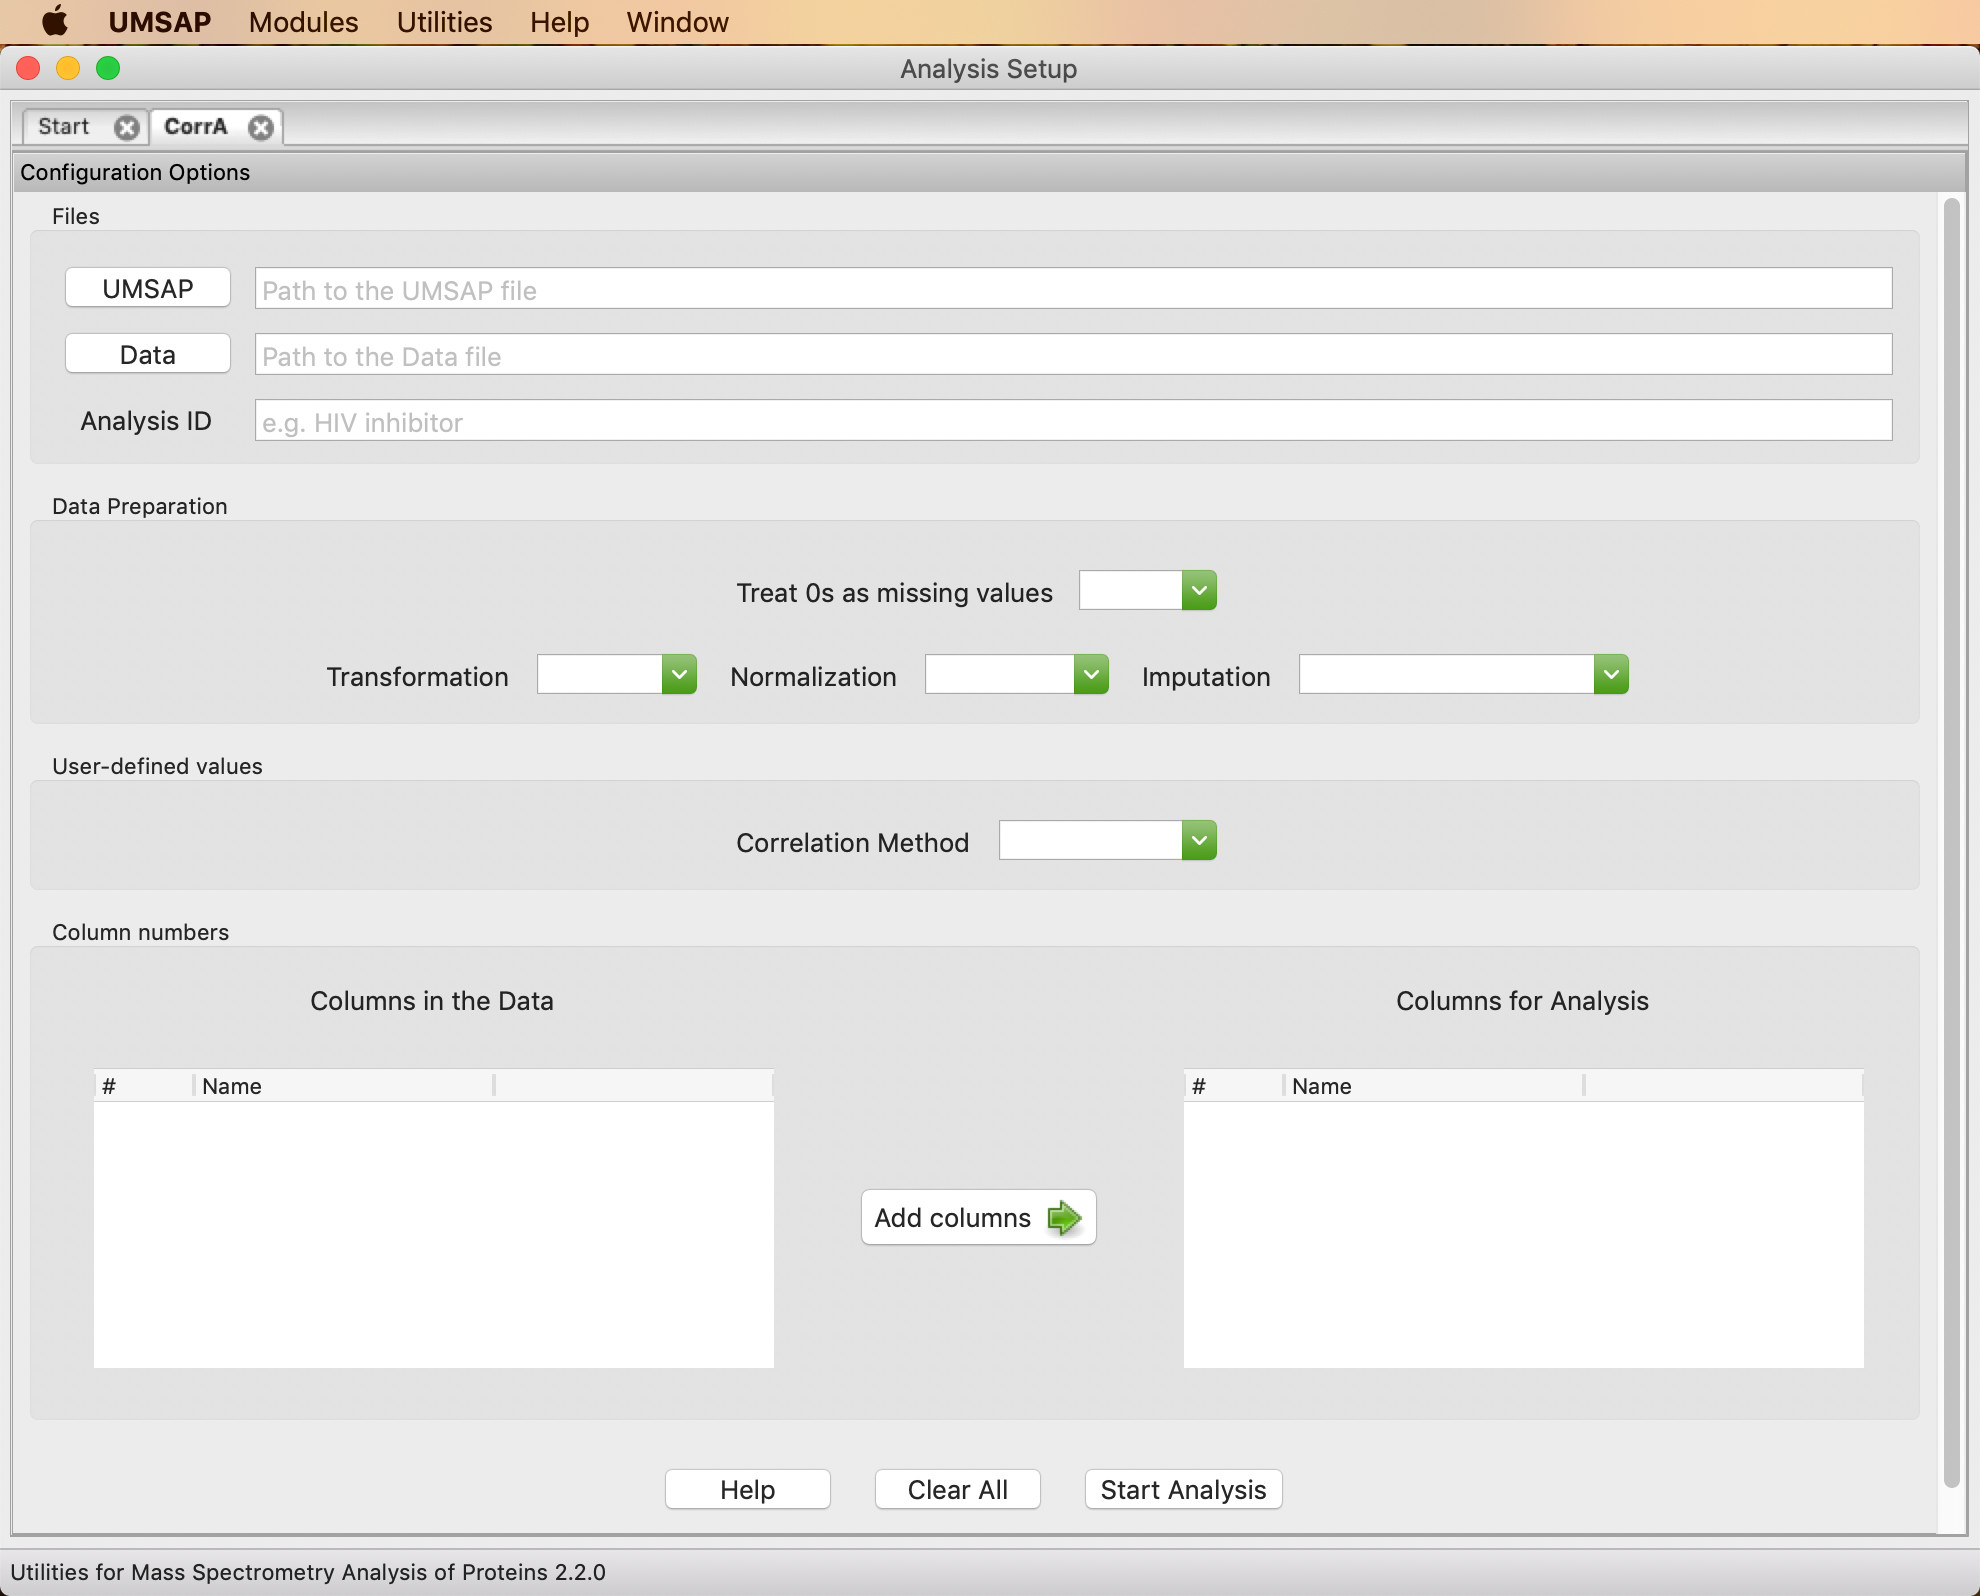
\includegraphics[width=0.7\textwidth]{./IMAGES/UTIL-CORR-WINDOW/util-corr.jpg}
    \caption[The Correlation Analysis tab]{\textbf{The Correlation Analysis tab.}
    This tab allows to perform a correlation analysis of the data contained in a
    given Data file.}
    \label{fig:utilCorrAnalysis}
    \vspace{-5pt}
\end{figure}

Section Files contains two buttons and a text field. Here users select the input
and output files for the analysis.

\num{1}. The button UMSAP allows selecting the location
and name of the umsap file. When selecting an already existing umsap file the operating
system will ask if it is ok to replace the file, the answer can be yes since UMSAP
will never overwrite or replace an umsap file. Instead, the new analysis will be
added to the already existing file. Only umsap files can be selected here.

\num{2}. The button Data allows selecting the input
data file that will be used for the analysis. The Data file is expected to be a
plain text file with tab separated columns and the name of the columns in the first
row of the file. In addition, columns to be analyzed must contain only numbers and
must be of the same length. Only .txt files can be selected here.

\num{3}. The text field Analysis ID allows providing an ID for the analysis
to be run. The date and time of the analysis will be automatically added to the
beginning of the name. For example, the Analysis ID \textit{First experiment} will
be transformed into \textit{20220504-124534 - First experiment}.

Section Data Preparation contains four dropdown boxes. Here users select how the data
in the Data file should be prepared before starting the analysis (\autoref{chap:dataPrep}).

\num{1}. The dropdown Treat \num{0}s as missing values allows defining how
to handle zero values present in the Data file. Selecting Yes results in UMSAP
replacing zero values with NA values. Selecting No results in UMSAP considering
zeros as valid values.

\num{2}. The dropdown Transformation allows selecting the Transformation method
to be applied to the data.

\num{3}. The dropdown Normalization allows selecting the Normalization method
to be applied to the data.

\num{4}. The dropdown Imputation allows selecting the Imputation method used
to replace missing values in the data.

Section User-defined values contains one dropdown box.

\num{1}. The dropdown Correlation Method allows selecting the correlation method
to use.

Section Column numbers contains two tables and a button. Here users select the columns
in the Data file to be used in the Correlation Analysis.

\num{1}. The table to the left will display the names of the columns present in the
selected Data file. The table is automatically filled once the Data file is selected.
Rows in the table can not be deleted, except in the case of loading a different Data
file or using the Clear All button at the bottom of the tab. Selected rows can be
copied (Cmd+C).

\num{2}. The table to the right will contain the columns in the Data file that will
be used for the Correlation Analysis. This table must contain at least two rows for
the analysis to proceed. Selected rows in this table can be deleted (Cmd+X)
and new rows can be pasted (Cmd+V). While pasting the rows, duplicate rows will be
discarded.
Importantly, the order of the rows and columns in the matrix containing the correlation
coefficients will be the same as the order of the columns in this table. Therefore,
users are advised to fill the table in such a way that replicates of the same experiment
are consecutive to each other in the table.

\num{3}. The button Add columns will add the selected rows in the left table to
the right table. The rows will be added to the right table in the same order as
they are selected in the left table. Duplicate rows will be silently discarded.

The bottom of the tab contains three buttons.

\num{1}. The button Help leads to an online tutorial about Correlation Analysis in
UMSAP.

\num{2}. The button Clear All will delete all user input from the tab.

\num{3}. The button Start Analysis starts the Correlation Analysis.

\section{The analysis}

First, UMSAP will check the validity of the user-provided input. Then, columns in
the right table are read from the Data file. The columns must contain only numbers
and the same amount of rows must be found in all columns. Failing to comply with
this will result in the program aborting the analysis. After this, all steps selected
in the Data Preparation section are carried out (\autoref{chap:dataPrep}). Finally,
the correlation coefficients are calculated using the selected method. If any of
the coefficients cannot be calculated, then the corresponding coefficient is set to NA.

\section{The results window}

The correlation coefficients resulting from a Correlation Analysis will be shown
as a color coded matrix (\autoref{fig:utilCorrAnalysisRes}). Values between \numrange{-1}{0}
will be shown in shades of red, \num{0} will be shown as white and values between
\numrange{0}{1} will be shown in shades of blue. NA values will be shown in green.
The columns and rows of the matrix are the column names used to calculate the correlation
coefficients. Information about a specific matrix element can be obtained by simply
placing the mouse pointer over the matrix element.

\begin{figure}[ht]
    \centering
    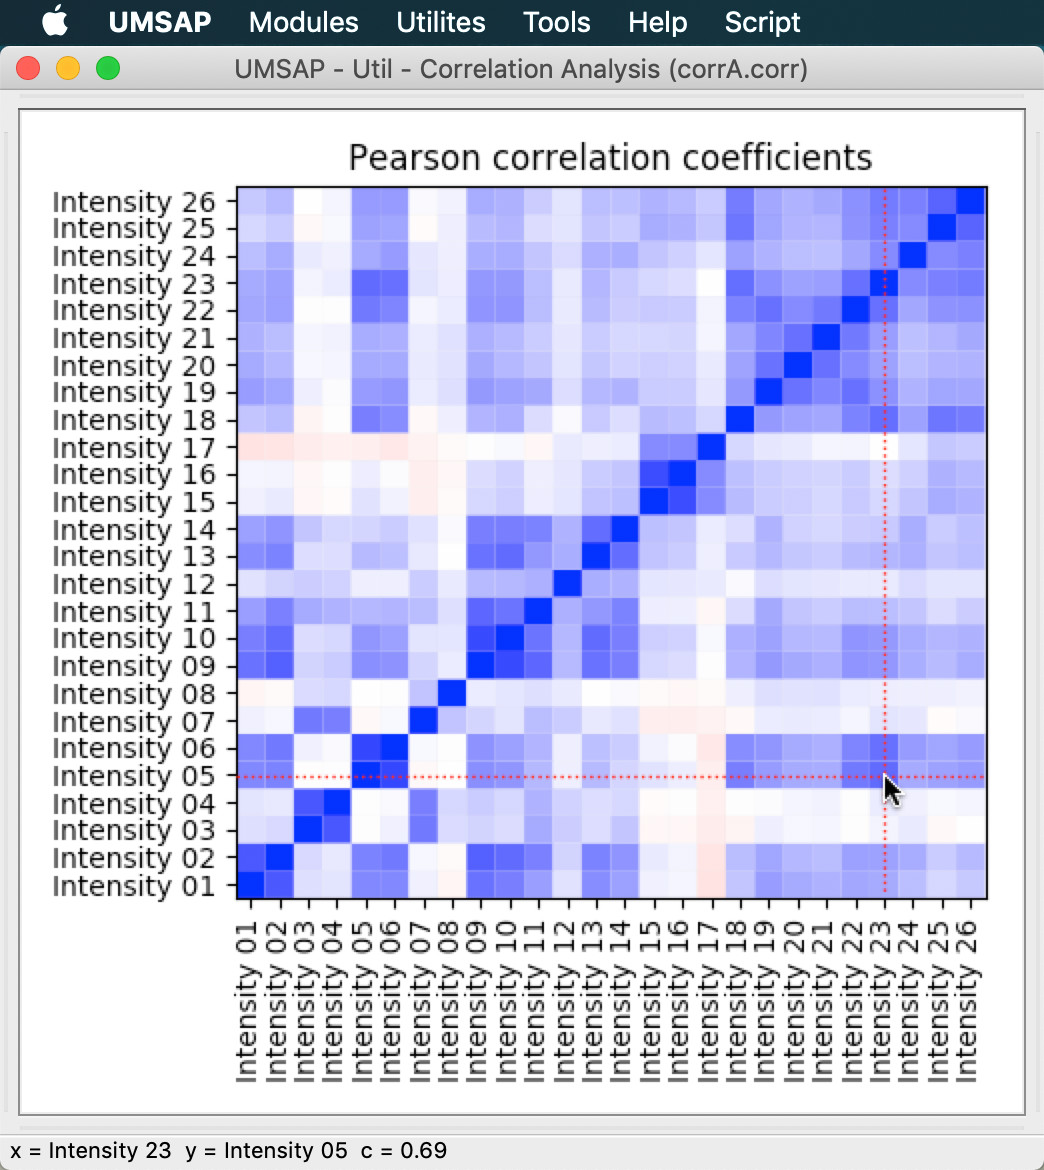
\includegraphics[width=0.7\textwidth]{./IMAGES/UTIL-CORR-WINDOW/util-corr-res.jpg}
    \caption[The Correlation Analysis result window]{\textbf{The Correlation Analysis
    result window.} The correlation coefficients are shown as a color coded matrix.
    Values between \numrange{-1}{0} are shown in shades of red, \num{0} is shown in
    white and values between \numrange{0}{1} in shades of blue. NA values are shown
    in green.}
    \label{fig:utilCorrAnalysisRes}
    \vspace{-5pt}
\end{figure}

\section{The Tools menu}

The menu Tools in the window showing the correlation coefficients allows viewing
any of the Correlation Analysis contained in the selected umsap file or to
modify the appearance of the displayed plot. For example, the column numbers can
be displayed instead of the column names or the color bar can be hidden. In addition,
only a subset of the columns can be shown using the Select Columns entry.

The menu Tools also allows duplicating the window (Cmd+D) for easier comparison of
two or more analysis, checking the Data Preparation steps of the analysis (Cmd+P),
creating an image of the plot (Cmd+I), exporting the correlation coefficient matrix
to a tab separated CSV file (Cmd+E) and resetting the zoom level of the plot (Cmd+Z).

